\begin{frame}
    \frametitle{Správce balíčků}
    \begin{definition}[Správce balíčků]
        \textbf{Správce balíčků} (package manager) je nástroj pro správu softwaru a jeho závislostí.\cite{wikipedia:správce_balíčků}
    \end{definition}
    \onslide<2->{Správce balíčků umožní publikaci, instalaci a aktualizaci vydání knihovny.}
\end{frame}

\begin{frame}{Správce balíčků - Ukázka NPM}
    \begin{figure}
        \centering
        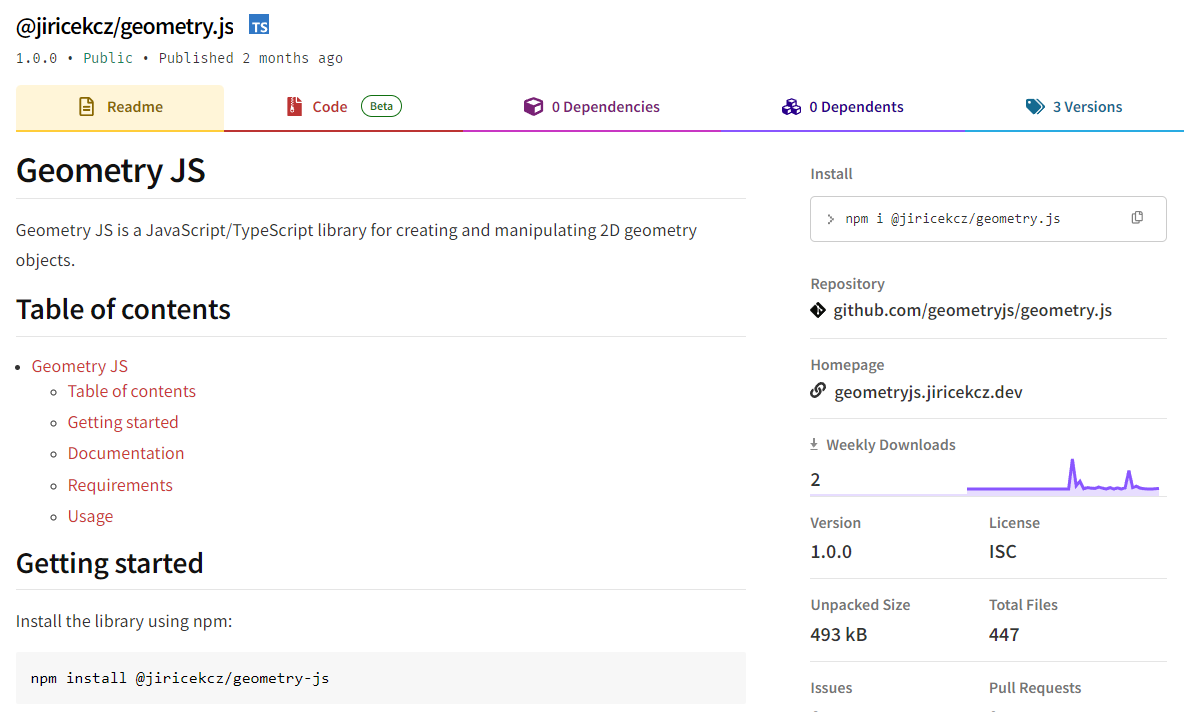
\includegraphics[height=0.718\textheight]{../resources/npm.png}
        \caption{Ukázka správce balíčků NPM}
    \end{figure}
\end{frame}